\documentclass{../lab_class}

\usepackage{fancyhdr}
\pagestyle{fancy}
\rhead{П.\,Ю. Смирнов, 687 гр.}
\lhead{Лабораторная работа № 3.1.1, МФТИ, осень 2017}

\newcommand{\magm}{\mathfrak{M}}

\begin{document}

{\Large 3.1.1 --  Магнитометр.}

\paragraph{Цель работы.}
Определить горизонтальную составляющую магнитного поля Земли и установить количественное соотношение между единицами электрического тока в системах СИ и СГС.
В работе используются: магнитометр, осветитель со шкалой, источник питания, вольтметр, электромагнитный переключатель, конденсатор, намагниченный стержень, секундомер, рулетка, штангенциркуль.

\begin{wrapfigure}[12]{r}{6cm}
\centering
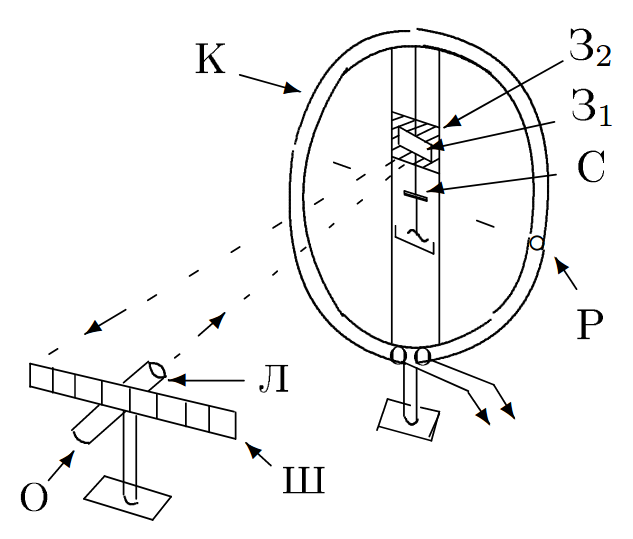
\includegraphics[width=5cm]{Fig1.png}
\caption{Схема магнитометра}
\end{wrapfigure}

\paragraph{Теоретическая часть.}
Магнитометр состоит из нескольких последовательно соединенных круговых витков, расположенных вертикально. В центре кольца на тонкой неупругой вертикальной нити подвешена короткая магнитная стрелка. В отсутствии других магнитных полей стрелка располагается по направлению горизонтальной составляющей земного магнитного поля $B_0$, т.~е. лежит в плоскости земного меридиана. Прибор настраивают с помощью двух световых зайчиков (зеркал), один из которых прикреплен к стрелке, а второй -- жестко к кольцу. Оба зеркала освещаются одним и тем же осветителем. Мы настраиваем прибор так, чтобы оба зайчика совпадали. При включении внешнего магнитного поля (например, путем создания тока в кольце ($B_2$) или внесения ферромагнитного стержня ($B_1$)) стрелка (и вместе с ней зайчик) отклоняется и направлена вдоль равнодействующей полей $B_0$ и $B_{\perp}$. 

Поле магнитного стержня есть
$$
	B_1 = \dfrac{\mu_0}{4\pi} \dfrac{\magm}{R^3},
$$
где $\magm$ -- магнитный момент стержня, $R$ -- радиус кольца. Поле же в центре кольца с током находим по закону Био и Савара:
$$
	B_2 = \dfrac{\mu_0 I}{2R} N.
$$
где $N$ -- число витков, $I$ -- сила тока. Измерив угол отклонения стрелки, мы можем связать поля:
$$
	B_{\perp} = B_0 \tan{\varphi}.
$$

\begin{wrapfigure}[12]{l}{6cm}
\centering
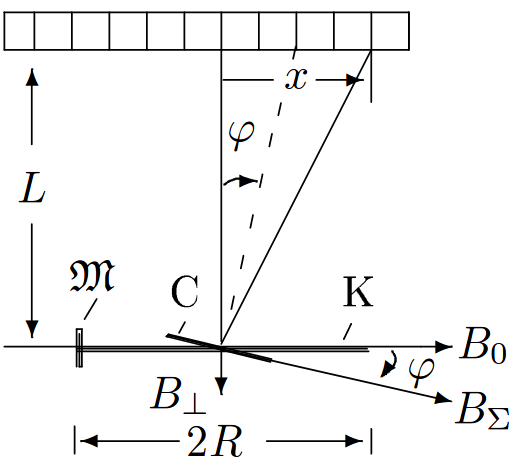
\includegraphics[width=5cm]{Fig2.png}
\caption{Схема измерения угла отклонения магнитной стрелки}
\end{wrapfigure}

Мы можем легко измерить горизонтальную составляющую магнитного поля Земли, если исключим неизвестный для нас магнитный момент используемого стержня. Для этого заметим, что такой стержень во внешнем магнитном поле может совершать малые (гармонические) колебания под действием механического момента $M_{\text{mech}} \simeq \magm B_0 \alpha$ с периодом $T = 2\pi \sqrt{ \dfrac{J}{\magm B_0} }$, где $J$ -- момент инерции стержня. Считая его цилиндром массой $m$, длиной $l$ и радиусом $r$, находим момент инерции: $J = m \left( \dfrac{l^2}{12} + \dfrac{r^2}{4} \right)$. Отсюда окончательно имеем:
$$
	B_0 = \dfrac{2\pi}{TR} \sqrt{ \dfrac{\mu_0 J L}{2\pi R x_1} }.
$$

Кроме того, мы можем также определить электродинамическую постоянную $c$:
$$
	c = 10 \dfrac{\{ I \}_{\text{СГС}}}{ \{ I \}_{\text{СИ}}}.
$$

В СИ ток, пропускаемый через магнитометр, можно определить через угол отклонения стрелки:
$$
	\{ I \}_{\text{СИ}} = \dfrac{2 B_0 R}{\mu_0 N} \tan{\varphi_2}.
$$
Одновременно измеряется ток в системе СГС. В секунду конденсатор $C$ перезаряжается $n$ раз, т.~о. через витки протекает ток
$$
	\{ I \}_{\text{СГС}} = C U n.
$$

\begin{wrapfigure}[12]{r}{6cm}
\centering
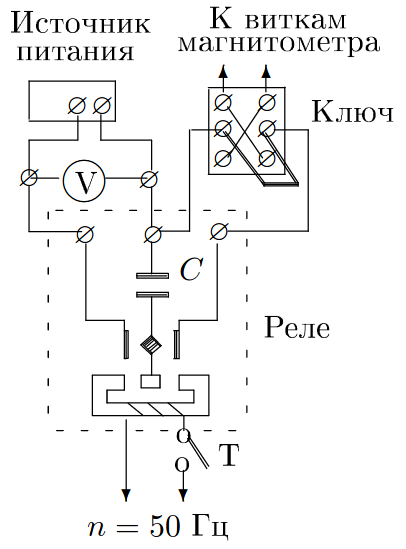
\includegraphics[width=5cm]{Fig3.png}
\caption{Схема питания катушки магнитометра}
\end{wrapfigure}

\paragraph{Горизонтальная составляющая магнитного поля Земли.}
Используя результаты измерений, мы легко находим, что $J \simeq 1.82 \times 10^{-7}$; отсюда получаем
$$
	B_0 \simeq 14.7 \; \smu \T.
$$

\begin{table}[H]
\centering
\begin{tabular}{|c|c|}
			\hline
	$R$, \cm & 25   \\ \hline
	$T$, \s  & 1.75 \\ \hline
	$l$, \cm & 2.41 \\ \hline
	$r$, \mm & 4.5  \\ \hline
	$m$, \g  & 2.87 \\ \hline
	$L$, \cm & 81   \\ \hline
	$x_1$, \cm & 11.3 \\ \hline	
	$N$, втк. & 34 \\ \hline
	$n$, \hz & 50 \\ \hline
	$C$, \cm & $9 \times 10^5$ \\ \hline
\end{tabular}
\caption{Измерения}
\end{table}

\paragraph{Электродинамическая постоянная.}
Найдем постоянный коэффициент в формуле для силы тока в СИ:
$$
	A = \dfrac{2 B_0 R}{\mu_0 N} \simeq 0.172.
$$

\begin{table}[H]
\centering
\begin{tabular}{|c|c|c|c|c|c|}
			\hline
	U, \V  & $\Delta x$, \cm & $\tan{\varphi}$ & $\{ I \}_{\text{СИ}}$, \sm \A & $\{ I \}_{\text{СГС}} \times 10^6$ & $c \times 10^{10}$ \\ \hline
	90 & 10.5 & 0.0648 & 11.1 & 13.5 & 1.2 \\ \hline
	90 & 11   & 0.0679 & 11.6 & 13.5 & 1.1 \\ \hline
	70 & 8    & 0.0494 & 8.5  & 10.5 & 1.2 \\ \hline
	70 & 8    & 0.0494 & 8.5  & 10.5 & 1.2 \\ \hline
	80 & 9    & 0.0555 & 9.55 & 12   & 1.2 \\ \hline
	80 & 9.5  & 0.0586 & 10.1 & 12   & 1.2 \\ \hline
	60 & 7.5  & 0.0463 & 7.96 & 9    & 1.1 \\ \hline
	60 & 7    & 0.0432 & 7.43 & 9    & 1.2 \\ \hline
\end{tabular}
\caption{Зайчик и конденсатор}
\end{table}
$$
	\then c \simeq 1.2 \times 10^9 \; \m \text{/} \s.
$$
\emph{Как объяснить расхождение в 2.5 раза?} Вероятно, неточной настройкой измерительных приборов.

\paragraph{Вывод.}
Относительно простое устройство позволило нам измерить магнитное поле Земли и, фактически, скорость света.

\end{document}